\documentclass{article} % For LaTeX2e
\usepackage{nips14submit_e,times}
\usepackage{hyperref}
\usepackage{url}
%\documentstyle[nips14submit_09,times,art10]{article} % For LaTeX 2.09
\usepackage{graphicx,subcaption}              % to include figures
\usepackage{epstopdf}
\usepackage{amsmath}               % great math stuff
\usepackage{amsfonts}              % for blackboard bold, etc
\usepackage{amsthm}                % better theorem environments

\usepackage{notoccite}
\usepackage[numbers,sort&compress]{natbib}
\usepackage{array}
\title{Multiple Sclerosis Lesion Segmentation in MRI Images }

\author{
Gautham Vasan \\
Department of Computing Science\\
University of Alberta\\
Edmonton, T6E2H2 \\
\texttt{vasan@ualberta.ca} \\
\And
Jared Rewerts \\
Department of Computer Engineering \\
University of Alberta \\Edmonton, T6E2H2 \\
\texttt{rewerts@ualberta.ca} \\
\And
Megha Panda \\
Department of Computing Science\\
University of Alberta \\Edmonton, T6E2H2 \\
\texttt{meghaanu@ualberta.ca} \\
\texttt{email} \\
\And
Parisa Mohebbi \\
Department of Computing Science \\
University of Alberta \\Edmonton, T6E2H2 \\
\texttt{mohebbi@ualberta.ca} \\
\And
Reza Sobhannejad \\
Department of Computing Science \\
University of Alberta \\Edmonton, T6E2H2 \\
\texttt{sobhanne@ualberta.ca} \\
\And
Sina Jalali  \\
Department of Computing Science \\
University of Alberta \\Edmonton, T6E2H2 \\
\texttt{jalali1@ualberta.ca} \\
}

% The \author macro works with any number of authors. There are two commands
% used to separate the names and addresses of multiple authors: \And and \AND.
%
% Using \And between authors leaves it to \LaTeX{} to determine where to break
% the lines. Using \AND forces a linebreak at that point. So, if \LaTeX{}
% puts 3 of 4 authors names on the first line, and the last on the second
% line, try using \AND instead of \And before the third author name.

\newcommand{\fix}{\marginpar{FIX}}
\newcommand{\new}{\marginpar{NEW}}

\nipsfinalcopy % Uncomment for camera-ready version

\begin{document}


\maketitle
% Abstract
\begin{abstract}
Medical Imaging is an emerging field that can help workload for medical professionals and increase outcomes for afflicted individuals. Our focus is on comparing classification techniques for Multiple Sclerosis lesions in order to find the most successful techniques. We also attempt to combine some techniques to improve detection success. Our results confirm the standard that Random Forest typically provides the best results, but that there are other options useful in segmenting lesions. Interestingly, Random Forest also tends to classify quicker than other algorithms, particularly when compared to SVM. This makes it the most practical in terms of accuracy and speed. 
\end{abstract}

%---------------------------------------- Introduction-------------------------------------------%
\section{Introduction}
%What is MS? Why it is an interesting problem? Problem definition and motivation. What are the challenges?
Multiple Sclerosis is a debilitating disease that affects the brain and spinal cord. Technically, MS is an autoimmune disease; the immune system attacks parts of the body, in this case, the protective covering of nerve fibers. If occurrences are bad enough, the nerves can build up scar tissue, which impedes nerve conduction. This scar tissue is what we refer to as lesions.

One of the most shocking aspects of Multiple Sclerosis is that it primarily affects individuals between the ages of 15 and 40. Women are also twice as likely to be affected by MS. Early detection is key to managing symptoms and controlling disease outcomes. Affected individuals can use exercise, cool temperatures and a balanced diet to help treat symptoms.

To detect Multiple Sclerosis lesions, scans are made of patient brains. Medical professionals analyze these scans, looking for signs of MS. These manual segmentation techniques have several drawbacks, not least among them the time input required by the medical professionals. Manual segmentation also has a high rate of error; only 70\% of lesions are properly detected [CITATION NEEDED]. Automatic segmentation techniques hope to improve these. 

One of the main challenges of automatic segmentation is the low lesion volume in patient brain matter. Typically, only a small percentage of the patients brain has lesions, which can make detecting them difficult. This also poses a problem when gathering positive examples of the lesion. The positive to negative ratio is much lower than in many other segmentation problem spaces. Further, since most patients have very little lesion tissue, over classification can be a problem with automated segmentation. If a healthy brain is scanned and processed, ideally, we would show no lesions. In practice, this is can be very difficult.


\subsection{Related Work}
Segmentation of Lesions in MRI images is an active area of research. The 3 main objectives are: 
\begin{enumerate}
  \item Extracting features that can differentiate healthy tissues from scar tissues, 
  \item Selecting the most relevant features that help achieve the task, and
  \item Improving the performance of the classification.
\end{enumerate} 

\subsubsection{Review of Segmentation Methods}
In MS lesion segmentation, the typical features are the intensity of each voxel in different modality images. Additionally, some methods like  \cite{commowick2009continuous}, combined K-NN based on intensities with a template-driven segmentation method to reduce false positives. Others like the method presented in \cite{zijdenbos2002automatic} used the probability of a voxel belonging to tissue class with help of an atlas. Intensity of the six neighbour voxels can be added to feature vector of a point which has been used with an ANN in \cite{younis2007ms}. In \cite{kroon2008multiple}, they used up to 255 features derived from applying different filters on images, and then with the help of principal component analysis (PCA), data is transformed to new orthogonal coordinates so the first column covers the greatest variance between data; hence, a simple thresholding on the first component of PCA can classify lesions. In \cite{geremia2011spatial}, random decision forest (RDF) is used with local (like intensity) and context-rich (will be discussed later) features. RDF has the advantage of automatically selecting the best features over other methods.

\subsubsection{ Exploring Combinations [PLEASE GIVE YOUR COMMENTS ON THIS PART] }
Lots of methods have been employed for lesion segmentation as mentioned before but no valid comparison is done to measure performance of different classifiers using different features. In this project we aim to compare various algorithm's efficiencies on the same data and feature sets to explore their properties in  lesion segmentation. We use Support Vector Machine (SVM), Neural Networks, K-Nearest Neighbors, Random Forest, Markov Random Field, and Logistic Regression as classifiers. For features, we use Haar-Like, image filters, LM filters, entropy, gaussian based, and atlas. In a broad sense, we tried to extract all possible features to see how the well-known classifiers operate based on them.

%------------------------------------------- Features ----------------------------------------------%
\section{Feature Detection}
%What is feature extraction? Why is it important? Reasons for using the particular features
Image analysis aims at reducing information to a subset that is relevant to the task in hand. Information reduction often happens gradually with information being reduced until the desired result is extracted from the data. \cite{toennies2012guide} The first level of reduction computes local features that
are assumed to pertain to objects of interest. 
\subsection{Context (Haar-Like Features)}
In the detection phase of the Viola-Jones object detection framework \cite{Viola-Jones}, a window of the target size is moved over the input image, and for each subsection of the image the Haar-like feature is calculated. This difference is then compared to a learned threshold that separates non-objects from objects. Because such a Haar-like feature is only a weak learner or classifier (its detection quality is slightly better than random guessing) a large number of Haar-like features are necessary to describe an object with sufficient accuracy. 

\begin{figure}[h]

\centering
\begin{subfigure}[b]{.4\linewidth}
\centering
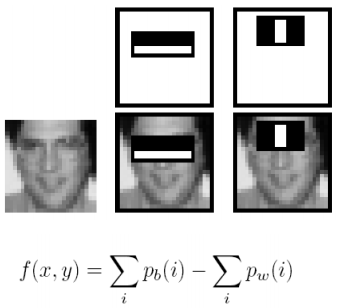
\includegraphics[scale=0.4]{haar}
\caption{ Calculation of Haar-like feature}
%\label{fig:subim1}
\end{subfigure}
\begin{subfigure}[b]{.4\linewidth}
\centering
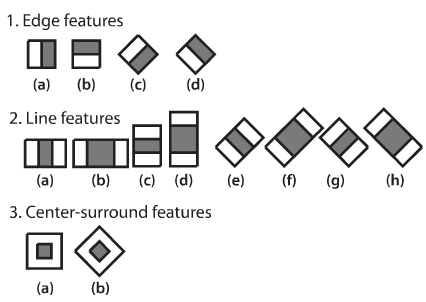
\includegraphics[scale=0.4]{HaarFeatures}
\caption{Different types of Haar-like Features}
%\label{fig:subim2}
\end{subfigure}

\caption{Haar-Like Features}
\end{figure}

\subsection{Image Filters}
Filtering is a technique used for modifying or enhancing an image. It can be used to emphasize certain features or remove other features in an image. In image processing filters are mainly used to suppress either the high frequencies in the image, i.e. smoothing the image, or the low frequencies, i.e. enhancing or detecting edges in the image. We extract the features through Linear filtering of the MRI image using convolution. 

\subsubsection{Leung-Malik (LM) Filter Bank}
We use the filter bank provided by the Visual Geometry Group at the University of Oxford [] to obtain a set of features. The LM set is a multi scale, multi orientation filter bank with 48 filters. It consists of first and second derivatives of Gaussians at 6 orientations and 3 scales making a total of 36; 8 Laplacian of Gaussian (LOG) filters; and 4 Gaussians. The filters occur at the basic scales $\sigma$ = {$\sqrt{2}$,2,2$\sqrt{2}$,4}. The Gaussians occur at the four basic scales while the 8 LOG filters occur at $\sigma$ and 3$\sigma$.

\begin{figure}[h]
\centering
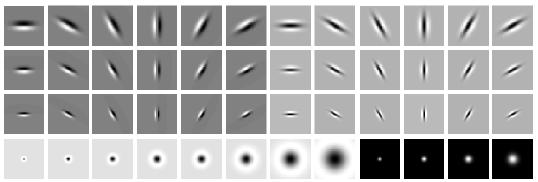
\includegraphics[scale=0.5]{lmfilters}
\caption{The LM filter bank has a mix of edge, bar and spot filters at multiple scales and orientations. It has a total of 48 filters}
\label{fig:LM filters}
\end{figure}

\subsection{Entropy \& Gaussian based Features)}

\subsection{Atlas Features}

All the features need to explained briefly with good images.

%------------------------------------------------ Classifiers ------------------------------------------%
\section{Classifiers}

Reasons for using each classification method. Brief description about them. No need for images here I guess.  

\subsection{Support Vector Machines}

\subsection{Neural Networks}

\subsection{k-Nearest Neighbours}

\subsection{Random Forests}
reason for using random forest instead of a single decision tree: decision trees are known to suffer from overfitting, so it is better to have a forest and ensemble many decision tree. based on \cite{geremia2011spatial}

\subsection{Markov Random Fields}

The basic principle of Markov Random Field is to treat the input image as a graph in which each voxel is a node and all the neighboring voxels are interconnected. In the case of foreground segmentation, two spatial nodes of foreground and background are added to the graph and edges between voxels. Each pair of nodes are assigned a weight equal to the probability that a given voxel belongs to either foreground or background. In graph theory, a cut is a partition of the vertices of a graph into two disjoint subsets. An st-cut is a graph cut comprising all directed edges from a node in a vertex set A to a node in its complement, $\overline{A}$, such that s $\epsilon$ A, t $\epsilon$ $\overline{A}$, and A is connected. The cost of a cut is simply defined as the sum of edge weights for the edges removed by the cut. The aim of this algorithm is to use a graph-cut to divide graph into two classes subject to the Min-Cut problem, i.e, to find the st-cut with minimal cost. The advantage of this method is that it considers the probabilities of its neighbours as a feature.

In this project, we trained a random forest (Claimed to be the best algorithm for lesion segmentation according to literature survey \cite{garcia2013review}) and used it to obtain initial probabilities of each voxel classified as a lesion. Subsequently, MRF is applied on the graph constructed using the weights,i.e., probabilities obtained from the classifier..


\subsection{Logistic Regression}

%-----------------------------------Experiment Design -------------------------------------------------------%
\section{Experiment Design}
Pipeline Diagram is required here

\subsection{Validation Measures}
For each pixel of the brain, our classifiers must label it as either lesion or healthy brain matter. Depending on the data set used, our ground truth source may be different. The MICCAI data set is provided by doctors and has also been cross referenced several times. The hope is that this increases the accuracy of the results. The MICCAI scan represent real brains. Brain Web on the other hand uses a simulated brain scan and places lesions in the simulated scans.

When comparing our output to the ground truth, we come up with 4 possibilities for each region of the brain scan:
\begin{enumerate}
  \item True Positive \newline
		The ground truth and our detection agrees the region is a lesion.
  \item True Negative \newline
  		The ground truth and our detection agrees the region is healthy.
  \item False Positive \newline
  		Our detection finds a lesion in a brain region, but the ground truth disagrees.
  \item False Negative \newline
  		The ground truth finds healthy brain, but our detection disagrees.
\end{enumerate} 
Taken together, these values can be used to analyze the performance of different classifiers. 
\subsubsection{Dice Score}
Dice is the primary metric we used to analyze algorithm performance. 

$$\frac{2*True Positive}{False Positive + False Negative + 2*True Positive}$$

One of the major benefits of Dice is that it heavily weights true positives. This makes it a very strict measure for a problem space like ours, where the amount of positive tissue is very low. 

As an example, consider scanning a brain that has a single tiny lesion. To get a perfect dice score, you must classify that lesion and only that lesion. Failing to classify that lesion will result in a score of 0. If you successfully classify the lesion, but also falsely classify surrounding tissue, the dice score will decrease rapidly. Since the healthy tissue heavily outweighs the lesions, it is easy to falsely classify a small amount of this healthy tissue as lesion.

There is one caveat to keep in mind when using Dice however. If we test against a healthy brain scan, Dice cannot be used to analyze our results. This is because there is no possibility of getting a true positive and so the result will always be 0.

\subsubsection{Accuracy}
Accuracy is good measure of how much brain matter we properly classify. Unlike Dice, accuracy weights true negatives evenly with true positives.

$$\frac{True Positive + True Negative}{False Positive + False Negative + True Positive + True Negative}$$

For our problem, accuracy usually isn't very useful. The reason for this is that true negatives are too common to be considered a reliable metric. For most brain scans, you could just classify the brain as healthy and the resulting accuracy would be good. We still use it though, as it can be useful when scanning healthy brains, which is where Dice fails.

\subsubsection{Sensitivity}

Sensitivity is similar to Dice in that it heavily weights true positives.

$$\frac{True Positive}{False Negative + True Positive}$$

Sensitivity affords no penalty to misclassifying healthy brain as lesion. This means a brain scan that is output as entirely lesion will do well on it. Despite this drawback, it can still be useful in situations that Dice is in.

\subsubsection{Detections}

As a simple evaluation measure, we count the number of properly classified lesions. A lesion is considered classified if we find even a single pixel of lesion within it. This makes it unreliable in terms of overall performance, but it is a valuable metric for basic testing of classifiers.

\subsection{Training and Test Data}
%BrainWeb and Miccai Challenge Data. Explain how sampling is done on data to train the classifier.
The quantitative analysis of the MRI images is done using data provided by two sources:
\begin{enumerate}
\item Brain Web - MS Lesion Brain Database, McGill University
\item MICCAI Challenge 2008 Dataset
\end{enumerate}

There exists no common ground truth or gold standard in most medical analysis tasks which results in an increasing need for validation of techniques. The Simulated Brain Database (SBD) acts as a stopgap solution to the validation problem. SBD is based on two anatomical models: (i) Normal brain and (ii) MS Lesion.  For both the models, full 3-dimensional data volumes have been simulated using three sequences (T1-, T2-, and proton-density- (PD-) weighted) and a variety of slice thicknesses, noise levels, and levels of intensity non-uniformity.  Unlike the vivo acquired data, here the ground truth is known which helps evaluating the various image analysis methods. 

The MICCAI challenge dataset is actual MRI image scans provided in 3 sequences - T1, T2 and Flair. The actual MRI image scans are obtained from Boston Children's Hospital (CHB) and University of North Carolina, Chapel Hill (UNC). The labels for the data are provided by two or more experts for each brain which results in a rough estimate for the presence of a lesion. We have 10 labeled brain volumes each from CHB and UNC as training data. Additionally, we have 18 unlabeled volumes from CHB and 10 unlabeled volumes from UNC as test data. The difficulty in using the MICCAI challege data is that:
\begin{enumerate}
\item Less than 0.1\% of the brain volume is lesions
\item Different MRI Scanning devices result in different quality of images
\item No uniformly accepted Ground Truth or Gold Standard for validation
\end{enumerate}

Since the datasets are heavily biased, we sample the data from one volume on the brain and test on an entirely different volume of the brain. The sampling is done usually in a ratio 1:2 to 1:7 between positive and negative samples of data, where positive samples are considered to be lesions. For testing the classifier, the features are extracted for every pixel and tested on the entire volume of a brain.  

% --------------------------------------- Results ----------------------------------------------------%
\section{Results}
Lots of Images! Table with comparative results. Explanation for why we get these results. 

\begin{center}
\centering
\begin{tabular}{ | m{7em} | m{2cm}| m{2cm} | m{2cm} | m{2cm} | } 
\hline
\textbf{Classifier} & \textbf{Dice Score} & \textbf{Accuracy} & \textbf{Sensitivity} & \textbf{Detection}\\ 
\hline
SVM & 0 & 0 & 0 & 0  \\ 
\hline
Neural Networks & 0 & 0 & 0 & 0 \\ 
\hline
k-Nearest Neighbours & 0 & 0 & 0 & 0 \\ 
\hline
Random Forest & 0 & 0 & 0 & 0 \\ 
\hline
MRF with RF & 0 & 0 & 0 & 0 \\ 
\hline
Logistic Regression & 0 & 0 & 0 & 0 \\ 
\hline
\end{tabular}
\end{center}

\subsection{State of the art results}
The best results for segmenting MS lesions reported until now comes from random forest algorithm explained in \cite{geremia2011spatial}. Their proposed method contains of 30 separated decision trees with maximum depth of 20; each tree has a lower bound for information gain which stops it from further growing. They used two types of features, local features which are intensities and context-rich features which combine intensity of a single voxel with distant regions. This method is tested on MICCAI grand challenge 2008 and they got a dice score of $39.39 \pm 18.4$. This result comes from doing a 3-fold cross-validation, meaning model is trained on two different brains and tested on the third one and the procedure repeats for three times.\\
The important thing they revealed about MS lesion segmentation task is its need of having as more comprehensive training set as possible. They demonstrated that classifier with their selected features cannot detect lesions in locations which are not represented in training data.

\subsection{Discussion}
Detailed analysis of the results we get from different results

%-------------------------------------- Conclusion ------------------------------------------%
\section{Conclusion}

% ---------------------------------------- Acknowledgements ----------------------------------%
\section{Acknowledgements}

%------------------------------------------- References ----------------------------------------%
\section{References}

\bibliography{bibliography}
\bibliographystyle{plain}

\end{document}
